\chapter{New Revolutions in Particle Physics: Basic Concepts}

These notes follow Leonard Susskind's tenth lecture, with curation by LazyingArt LLC. The lecture begins as a deliberate reset. The previous account of how the Lagrangian leads to particle interactions was not yet sharp enough, so we go back and rebuild the bridge from the beginning: first least action for an ordinary particle, then least action for a field, then Feynman's rule for amplitudes, and only after that the practical route to propagators, vertices, and Feynman diagrams.

\section{Why Return to the Path Integral}

The lecture opens with a correction of emphasis. We are still thinking about quantum field theory, but not yet about the empirical catalog of particles. The point is to understand why the Lagrangian is not just a formal bookkeeping device. In this lecture it becomes the object from which we read amplitudes, and the path integral is presented as the most direct route from the Lagrangian to Feynman diagrams.

The organizing thought is classical in origin. Feynman's formulation is introduced as the quantum-mechanical version of the principle of least action. The lecture therefore begins by backing up to the classical action principle and then rebuilding the quantum story in that order. That order matters. If we begin instead with finished Feynman rules, the physical motivation is lost.

\section{From Classical Particle Motion to Classical Field Action}

For an ordinary Newtonian particle, the Lagrangian is a function of the coordinates and their time derivatives. The action is the integral of the Lagrangian along a trajectory:
\begin{equation}
S=\int \mathcal{L}(x,\dot{x})\,dt.
\end{equation}
Every trajectory from one spacetime point to another carries such an action, whether or not it is the true classical trajectory. The classical trajectory is the one singled out, in the lecture's language, by minimizing the action.

\begin{figure}[h]
\centering

\includegraphics[width=0.72\textwidth]{lecture_10_figure_02.png}

\begin{tikzpicture}[scale=0.9]
\draw[->] (0,0) -- (5.2,0) node[right] {$x$};
\draw[->] (0,0) -- (0,3.2) node[above] {$t$};
\draw[thick] (0.7,0.5) .. controls (1.5,1.0) and (2.3,1.7) .. (4.2,2.7);
\fill (0.7,0.5) circle (2pt);
\fill (4.2,2.7) circle (2pt);
\end{tikzpicture}
\caption{Action integral for a particle trajectory. The lecture frame is kept as documentary evidence, and the schematic curve below echoes the orbit picture carried on the board.}
\end{figure}

From this one derives differential equations, namely the classical equations of motion. The lecture does not stop to rederive them, and neither should we. The point here is to keep in view the structure: Lagrangian, then action, then the classical path.

Now the same structure is carried over to field theory, but the object is different. Instead of a worldline, we have a spacetime region between an initial time and a final time. Instead of a particle coordinate, we have fields. The Lagrangian depends on the field and its spacetime derivatives:
\begin{equation}
\mathcal{L}=\mathcal{L}\!\left(\phi,\partial_\mu\phi\right).
\end{equation}
In the lecture this is written in compact board form as \(\mathcal{L}\!\left(\phi,\frac{\partial\phi}{\partial x^\mu}\right)\). One further requirement, stated explicitly, is that the Lagrangian be a Lorentz scalar.

\begin{figure}[h]
\centering

\includegraphics[width=0.62\textwidth]{lecture_10_figure_03.png}
\caption{Lagrangian as a function of field and spacetime derivatives.}
\end{figure}

The action is now integrated over spacetime rather than along a single orbit:
\begin{equation}
S[\phi]=\int d^4x\,\mathcal{L}(\phi,\partial_\mu\phi).
\end{equation}
The analog of fixing the endpoints of a particle path is to fix the entire field on an initial time slice and on a final time slice. The field configuration in between is then determined classically by the same least-action idea.

\begin{figure}[h]
\centering
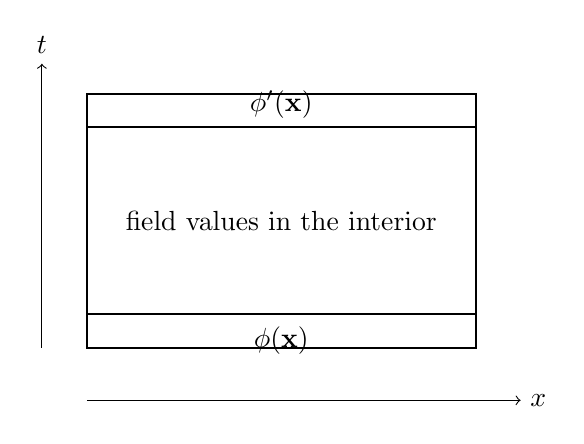
\begin{tikzpicture}[scale=0.95]
\draw[->] (-0.6,0) -- (-0.6,3.8) node[above] {$t$};
\draw[->] (0,-0.7) -- (5.8,-0.7) node[right] {$x$};
\draw[thick] (0,0) rectangle (5.2,3.4);
\draw[thick] (0,0.45) -- (5.2,0.45);
\draw[thick] (0,2.95) -- (5.2,2.95);
\node at (2.6,0.1) {$\phi(\mathbf{x})$};
\node at (2.6,3.25) {$\phi'(\mathbf{x})$};
\node at (2.6,1.7) {field values in the interior};
\end{tikzpicture}
\caption{The field-theory analog of fixed endpoints: initial and final field configurations on two time slices, with a spacetime region in between.}
\end{figure}

We may phrase the classical field problem this way: given \(\phi(\mathbf{x})\) initially and \(\phi'(\mathbf{x})\) finally, is there a field configuration in the slab between them? Classically the answer is yes, and the correct one is selected by minimizing the action over the spacetime region.

\section{Particle Amplitudes and Feynman's Rule}

At this point the lecture pivots from equations of motion to amplitudes. For a particle, the natural quantum question is not which path it follows, but what the amplitude is to start at one spacetime point and later be found at another. That amplitude is a complex number. Its magnitude squared is the corresponding probability:
\begin{equation}
P=|\mathcal{A}|^2=\mathcal{A}\mathcal{A}^*.
\end{equation}

Feynman's rule is then stated in its simplest form. Take any trajectory from \((x,t)\) to \((x',t')\), compute its action, and assign to that trajectory the phase
\begin{equation}
e^{-iS/\hbar}.
\end{equation}
The lecture frame preserves the board-level form of this statement, even though the \(\hbar\) is restored from the transcript rather than from the chalk itself.

\begin{figure}[h]
\centering

\includegraphics[width=0.70\textwidth]{lecture_10_figure_04.png}

\begin{tikzpicture}[scale=0.9]
\draw[->] (0,0) -- (4.8,0) node[right] {$x$};
\draw[->] (0,0) -- (0,3.2) node[above] {$t$};
\draw[thick] (1.0,0.6) .. controls (1.5,2.4) and (2.7,2.8) .. (2.3,1.3)
                     .. controls (2.0,0.6) and (3.0,0.9) .. (4.0,2.5);
\fill (1.0,0.6) circle (2pt);
\fill (4.0,2.5) circle (2pt);
\end{tikzpicture}
\caption{Phase factor associated with a particle path. The lecture frame is kept, and the small path sketch is redrawn schematically below.}
\end{figure}

The amplitude is then the sum over all trajectories:
\begin{equation}
\mathcal{A}(x,t\to x',t')=\sum_{\text{paths}} e^{-iS/\hbar}.
\end{equation}
In the nonrelativistic case the lecture reminds us that we do not allow paths to loop backward in time. What matters for the present argument is that every possible path contributes, not only the classical one.

\subsection{Question \& Answer}

\paragraph{Question.} If each contribution has magnitude one, why does the sum not immediately blow up?

\paragraph{Answer.} Because the contributions are complex phases. They do not add as positive real numbers. They lie on the unit circle and oscillate, so different paths cancel one another. The lecture insists on this point: the crucial mechanism is cancellation, not term-by-term decay.

\paragraph{Question.} Then why does classical mechanics ever emerge?

\paragraph{Answer.} Because the paths near a classical path tend to cancel least. In the lecture's language the dominant paths are those of minimum action; in cleaner modern language one would say stationary action. Either way, the classical limit comes from the special set of paths for which the phase varies least rapidly.

\section{From Trajectories to Field Histories}

We now make the essential replacement. In field theory the analog of a particle path is not another geometric trajectory in spacetime. The lecture corrects that idea explicitly. The trajectory is replaced by a history: a full assignment of field values throughout the spacetime region between the initial and final slices.

So we begin with an initial field configuration \(\phi(\mathbf{x})\) and a final field configuration \(\phi'(\mathbf{x})\). The amplitude is obtained by summing over all interpolating field histories:
\begin{equation}
\mathcal{A}\big[\phi(\mathbf{x})\to \phi'(\mathbf{x})\big]
=\sum_{\text{histories}} e^{-iS[\phi]/\hbar},
\qquad
S[\phi]=\int d^4x\,\mathcal{L}(\phi,\partial_\mu\phi).
\end{equation}

The lecture keeps this at a deliberately heuristic level. We are not trying to give a rigorous measure-theoretic construction. We are trying to preserve the physical picture. A history means the values of the field everywhere in the spacetime slab. Every such history, whether or not it satisfies the classical field equations, carries an action, and therefore a phase. The amplitude between the boundary configurations is the sum of all those phases.

This is the first place where the particle and field viewpoints can be seen to be genuinely complementary. The particle story asks for amplitudes from one point to another. The field story asks for amplitudes from one whole field configuration to another. The lecture insists that these are not two different theories; they are two readings of the same underlying object.

\section{Discretizing Spacetime to Make Sense of the Path Integral}

The next move is practical. A continuum sum over all histories is hard to define directly, so spacetime is chopped into small cells. The field is then represented by its value in each cell. The lecture is careful here because it is correcting an earlier oversimplification.

What was said before was ``one plus the Lagrangian'' in each cell. Then the lecture corrects this: it should really be the action in each cell, not the bare Lagrangian. If the cell has spacetime volume \(a^4=\Delta x\,\Delta y\,\Delta z\,\Delta t\), then the action in the \(i\)-th cell is
\begin{equation}
A_i=\mathcal{L}_i\,a^4.
\end{equation}
Because the cell is small, \(A_i\) is small. This is where the heuristic comparison
\begin{equation}
1+\epsilon \approx e^\epsilon
\end{equation}
enters the lecture. It is used only as motivation. The correct form is exponential from the start:
\begin{equation}
e^{-\frac{i}{\hbar}\sum_i A_i}
=
\prod_i e^{-iA_i/\hbar}.
\end{equation}
This is the key identity. The exponential of the total action becomes a product of exponential factors, one factor for each cell.

\begin{figure}[h]
\centering
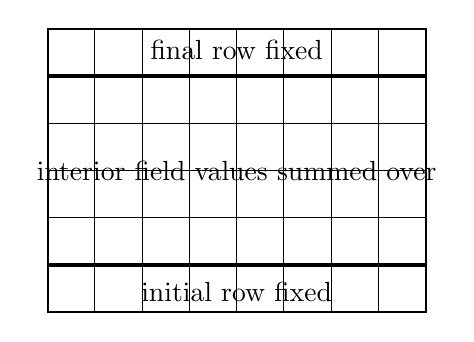
\begin{tikzpicture}[scale=0.75]
\draw[step=0.8,thin] (0,0) grid (6.4,4.8);
\draw[thick] (0,0) rectangle (6.4,4.8);
\draw[very thick] (0,0.8) -- (6.4,0.8);
\draw[very thick] (0,4.0) -- (6.4,4.0);
\node at (3.2,0.35) {initial row fixed};
\node at (3.2,4.45) {final row fixed};
\node at (3.2,2.4) {interior field values summed over};
\end{tikzpicture}
\caption{A lattice-like spacetime discretization. The first and last rows encode the boundary data; the interior is summed over.}
\end{figure}

For a fixed history, one multiplies together the phase factors from all cells. Then one sums over all ways of assigning field values to the interior cells, with the first and last rows fixed by the initial and final conditions.

\subsection{Question \& Answer}

\paragraph{Question.} Must the histories be continuous?

\paragraph{Answer.} No. The lecture answers this very emphatically. Once spacetime is discretized, continuity is no longer the right requirement. We assign field values to cells and sum over all assignments. There is no restriction to nearly smooth histories. Quantum fields, as the lecture puts it, jiggle a great deal.

\paragraph{Question.} Then what happens to derivatives on the lattice?

\paragraph{Answer.} We do not sum over derivatives independently. We sum over field values. Derivatives are then represented by differences between neighboring cells. Schematically,
\begin{equation}
\partial_\mu \phi(x)\ \longrightarrow\ \frac{\phi(x+\hat\mu)-\phi(x)}{a}.
\end{equation}
The lecture does not fix a single convention in detail; the point is simply that derivatives become neighbor-to-neighbor differences.

This is also where the lecture briefly gestures toward lattice quantum field theory as a real computational enterprise. The notes should preserve the point but not let it overwhelm the present chapter: the lattice is introduced here mainly to give concrete meaning to the path integral.

\section{Reading Particle Propagation Out of the Quadratic Terms}

Now the lecture returns from fields to particles. Fields are taken as shorthand for creation and annihilation operators, so products of fields can be read as particle processes. If we keep only the quadratic terms, we isolate the part of the theory responsible for propagation.

On the lattice, derivative terms couple neighboring cells. The simplest model of the structure is a finite difference:
\begin{equation}
\bigl(\phi(x)-\phi(x')\bigr)^2
=
\phi(x)^2+\phi(x')^2-2\phi(x)\phi(x').
\end{equation}
Here \(x\) and \(x'\) denote neighboring lattice sites. The cross term couples neighboring cells and is interpreted in the lecture as a hop from one box to the next. The same-site terms already tell us that ``standing still'' is also part of the quadratic story.

To isolate the particle motion, the lecture focuses schematically on nearest-neighbor cross terms of the form
\begin{equation}
\sum_{\langle x,x'\rangle}\phi(x)\phi(x').
\end{equation}
Then one expands the exponential:
\begin{align}
\exp\!\left[-i\sum_{\langle x,x'\rangle}\phi(x)\phi(x')\right]
&=
1
-i\sum_{\langle x,x'\rangle}\phi(x)\phi(x')
-\frac{1}{2!}\left(\sum_{\langle x,x'\rangle}\phi(x)\phi(x')\right)^2
+\cdots .
\end{align}
This should be read cautiously. The lecture is qualitative here. The coefficients and omitted local terms are not the point; the combinatorics is the point.

A single factor \(\phi(x)\phi(x')\) gives one elementary hop. A product of two such factors can give a two-step path. Higher powers produce longer chains. The coefficient of a particular chain is read off from the expansion, with factorials and powers of \(i\) included exactly as they arise from the exponential.

\begin{figure}[h]
\centering
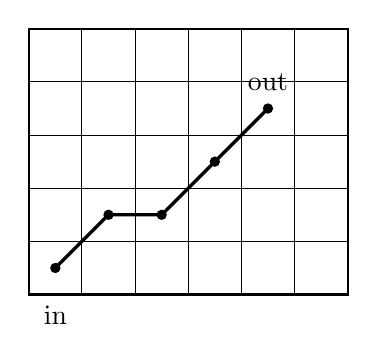
\begin{tikzpicture}[scale=0.75]
\draw[step=0.9,thin] (0,0) grid (5.4,4.5);
\draw[thick] (0,0) rectangle (5.4,4.5);
\fill (0.45,0.45) circle (2.5pt);
\fill (1.35,1.35) circle (2.5pt);
\fill (2.25,1.35) circle (2.5pt);
\fill (3.15,2.25) circle (2.5pt);
\fill (4.05,3.15) circle (2.5pt);
\draw[very thick] (0.45,0.45) -- (1.35,1.35) -- (2.25,1.35) -- (3.15,2.25) -- (4.05,3.15);
\node at (0.45,-0.35) {in};
\node at (4.05,3.6) {out};
\end{tikzpicture}
\caption{A schematic chain of nearest-neighbor hops. Higher-order terms in the expansion build long-distance propagation from local links.}
\end{figure}

The lecture also emphasizes a combinatorial rule: no dangling ends are allowed except where we explicitly insert particles in the initial state or remove them in the final state. This is the mechanism by which local hop terms are stitched together into actual propagators.

The quadratic theory also contains the mass term
\begin{equation}
\frac{1}{2}m^2\phi^2.
\end{equation}
In the lecture this is interpreted as a rule that does not move the particle at all. It annihilates and recreates it at the same site, thereby weighting a path without changing its position. This is how mass enters the path sum.

\subsection{Question \& Answer}

\paragraph{Question.} How do local nearest-neighbor terms build a long-distance propagator without leaving illegal loose ends behind?

\paragraph{Answer.} By going to higher orders in the exponential expansion. A single nearest-neighbor factor gives only one hop. A product of two can give two hops. A product of three can give a chain of three hops, and so on. The contributing terms are precisely those in which intermediate endpoints are paired off, leaving only the initial and final insertion points exposed.

\paragraph{Question.} What about paths that run backward in time?

\paragraph{Answer.} In the relativistic theory they are allowed. The lecture gives two equivalent readings. One may either say that a segment literally goes backward in time, or one may read the same graph forward in time as a particle-antiparticle pair being created, with the antiparticle annihilating the original particle. The second reading is often the more physical one.

\section{Interactions, Vertices, and the Perturbative Expansion}

Once the quadratic terms are understood, the lecture turns to higher powers of the field. These are the interaction terms. A cubic term
\begin{equation}
g_3\phi^3
\end{equation}
allows one particle to turn into two, or two into one, or three to be created, or three to be annihilated. A quartic term
\begin{equation}
g_4\phi^4
\end{equation}
gives four-legged events: two in and two out, one in and three out, three in and one out, or purely virtual four-particle creation and annihilation processes.

The important structural point is that the same exponential expansion that generated chains of hops now also generates vertices. A graph with one cubic insertion can split a worldline into two. A graph with two cubic insertions can split and then rejoin. The lecture gives the familiar physical example: an electron propagating from one point to another can emit a photon and later reabsorb it. That process is part of the amplitude for the electron to propagate.

We can now say explicitly what the lecture means by the equivalence of Lagrangian language and Feynman-diagram language. The quadratic terms define propagators. The higher-order terms define vertices. The diagrams are not extra physics added on top of the Lagrangian. They are a shorthand way of reading what the Lagrangian already says can happen.

Conservation laws also emerge in this language. The lecture recalls an earlier point: when one sums or integrates over all possible spacetime positions of a vertex, processes that violate energy or momentum conservation cancel out. In that sense conservation is not imposed by hand on each diagram separately. It emerges from the full spacetime sum over where the interaction could occur.

A simple worked example appears at the end of the lecture in the language of quantum electrodynamics. The basic interaction is the emission or absorption of a photon by an electron. The coupling is the electric charge \(e\). The lowest-order electron-photon scattering graph has two such vertices, so the amplitude scales as
\begin{equation}
\mathcal{A}_{\mathrm{QED,\,lowest}}\propto e^2.
\end{equation}
The probability therefore scales as
\begin{equation}
P_{\mathrm{QED,\,lowest}}\propto e^4.
\end{equation}
More complicated graphs carry extra powers of \(e\), so when \(e\) is small they are suppressed. This is the perturbative logic.

One must also keep the order of operations straight. We do not square each graph separately and then add. We add amplitudes first and only then square. Thus interference terms are essential:
\begin{equation}
\mathcal{A}_{\mathrm{total}}=\sum_r \mathcal{A}_r,
\qquad
P=\left|\sum_r \mathcal{A}_r\right|^2.
\end{equation}

\subsection{Question \& Answer}

\paragraph{Question.} Where do the coupling constants come from?

\paragraph{Answer.} Sometimes symmetries relate them, but in general the lecture says plainly that their values come from experiment. The Lagrangian is partly dictated by theoretical structure and partly by measured input.

\paragraph{Question.} Then why is this huge sum computationally useful at all?

\paragraph{Answer.} Because each additional interaction vertex contributes another power of the appropriate coupling. Schematically, if a diagram has \(V_3\) cubic vertices and \(V_4\) quartic vertices, then
\begin{equation}
\mathcal{A}_{\mathrm{diagram}}\propto g_3^{V_3}g_4^{V_4}\cdots .
\end{equation}
When the couplings are small, the simpler diagrams dominate and the more elaborate ones are progressively smaller. This does not solve every convergence problem, but it explains why perturbation theory has a chance to work.

The lecture closes by widening the lens once more. There are two ways to talk about the same physics. One may describe a process as a sum over field histories between fixed initial and final field configurations. Or one may describe it as a sum over particle processes built from propagators and vertices. The Lagrangian is useful in both languages. It is the single compact object that stores the rules for both.

\section{Summary}

The lecture has a very definite arc. We go back to the classical action only in order to come forward again to quantum amplitudes. For a particle, the action weights every trajectory by a phase. For a field, the same idea becomes a sum over histories. To make that sum concrete, we discretize spacetime into cells, attach an action to each cell, and rewrite the exponential of the total action as a product over the lattice. From the quadratic terms we read propagation, from the mass term we read same-site weighting, and from higher powers such as \(\phi^3\) and \(\phi^4\) we read interaction vertices. In this way the Lagrangian becomes both a field-theoretic action and a catalogue of particle processes, and the path integral becomes the bridge between the two descriptions.